\documentclass[11pt]{article}

% Change "review" to "final" to generate the final (sometimes called camera-ready) version.
% Change to "preprint" to generate a non-anonymous version with page numbers.
\usepackage[review]{acl}

% Standard package includes
\usepackage{times}
\usepackage{fancyvrb}
\usepackage{fvextra}
\usepackage{latexsym}
\usepackage{amsmath}
% For proper rendering and hyphenation of words containing Latin characters (including in bib files)
\usepackage[T1]{fontenc}
% For Vietnamese characters
% \usepackage[T5]{fontenc}
% See https://www.latex-project.org/help/documentation/encguide.pdf for other character sets

% This assumes your files are encoded as UTF8
\usepackage[utf8]{inputenc}

\usepackage{booktabs}
\usepackage{graphicx}
\usepackage{multirow}
\usepackage{array}
\usepackage[table]{xcolor}  % 颜色 + 表格单元格背景
\usepackage{enumitem}

% This is not strictly necessary, and may be commented out,
% but it will improve the layout of the manuscript,
% and will typically save some space.
\usepackage{microtype}

% This is also not strictly necessary, and may be commented out.
% However, it will improve the aesthetics of text in
% the typewriter font.
\usepackage{inconsolata}

%Including images in your LaTeX document requires adding
%additional package(s)
\usepackage{graphicx}

% If the title and author information does not fit in the area allocated, uncomment the following
%
%\setlength\titlebox{<dim>}
%
% and set <dim> to something 5cm or larger.

\title{RetailBench: Evaluating Long-Horizon Autonomous Decision-Making and Strategy Stability of LLM Agents in Realistic Retail Environments}

% Author information can be set in various styles:
% For several authors from the same institution:
% \author{Author 1 \and ... \and Author n \\
%         Address line \\ ... \\ Address line}
% if the names do not fit well on one line use
%         Author 1 \\ {\bf Author 2} \\ ... \\ {\bf Author n} \\
% For authors from different institutions:
% \author{Author 1 \\ Address line \\  ... \\ Address line
%         \And  ... \And
%         Author n \\ Address line \\ ... \\ Address line}
% To start a separate ``row'' of authors use \AND, as in
% \author{Author 1 \\ Address line \\  ... \\ Address line
%         \AND
%         Author 2 \\ Address line \\ ... \\ Address line \And
%         Author 3 \\ Address line \\ ... \\ Address line}

% \author{First Author \\
%   Affiliation / Address line 1 \\
%   Affiliation / Address line 2 \\
%   Affiliation / Address line 3 \\
%   \texttt{email@domain} \\\And
%   Second Author \\
%   Affiliation / Address line 1 \\
%   Affiliation / Address line 2 \\
%   Affiliation / Address line 3 \\
%   \texttt{email@domain} \\}

% \author{
%  \textbf{First Author\textsuperscript{1}},
%  \textbf{Second Author\textsuperscript{1,2}},
%  \textbf{Third T. Author\textsuperscript{1}},
%  \textbf{Fourth Author\textsuperscript{1}},
% \\
%  \textbf{Fifth Author\textsuperscript{1,2}},
%  \textbf{Sixth Author\textsuperscript{1}},
%  \textbf{Seventh Author\textsuperscript{1}},
%  \textbf{Eighth Author \textsuperscript{1,2,3,4}},
% \\
%  \textbf{Ninth Author\textsuperscript{1}},
%  \textbf{Tenth Author\textsuperscript{1}},
%  \textbf{Eleventh E. Author\textsuperscript{1,2,3,4,5}},
%  \textbf{Twelfth Author\textsuperscript{1}},
% \\
%  \textbf{Thirteenth Author\textsuperscript{3}},
%  \textbf{Fourteenth F. Author\textsuperscript{2,4}},
%  \textbf{Fifteenth Author\textsuperscript{1}},
%  \textbf{Sixteenth Author\textsuperscript{1}},
% \\
%  \textbf{Seventeenth S. Author\textsuperscript{4,5}},
%  \textbf{Eighteenth Author\textsuperscript{3,4}},
%  \textbf{Nineteenth N. Author\textsuperscript{2,5}},
%  \textbf{Twentieth Author\textsuperscript{1}}
% \\
% \\
%  \textsuperscript{1}Affiliation 1,
%  \textsuperscript{2}Affiliation 2,
%  \textsuperscript{3}Affiliation 3,
%  \textsuperscript{4}Affiliation 4,
%  \textsuperscript{5}Affiliation 5
% \\
%  \small{
%    \textbf{Correspondence:} \href{mailto:email@domain}{email@domain}
%  }
% }

\begin{document}
\maketitle
\begin{abstract}
Large Language Model (LLM)-based agents have achieved notable success on short-horizon and highly structured tasks, yet their ability to maintain coherent decision-making over long horizons in realistic and dynamic environments remains an open challenge. We introduce \textit{RetailBench}, a high-fidelity benchmark designed to evaluate long-horizon autonomous decision-making in realistic commercial scenarios, where agents must operate under stochastic demand and evolving external conditions.

We further propose the \textit{Evolving Strategy \& Execution} framework, which separates high-level strategic reasoning from low-level action execution, enabling adaptive and interpretable strategy evolution over time. This design is motivated by the observation that long-horizon tasks require strategies to be revised at a different temporal scale than action execution. Experiments on eight state-of-the-art LLMs across progressively challenging environments show that, in our evaluated settings, our framework is associated with higher mean operational stability and efficiency metrics compared to day-level Reflection baselines. However, performance degrades substantially as task complexity increases, and all models remain substantially below heuristic upper bounds. These observations suggest challenges that current LLMs face in long-horizon, multi-factor decision-making within the RetailBench environment\footnote{Due to computational constraints, our current evaluation uses a limited number of random seeds (three runs per setting); reported performance differences should be interpreted as preliminary observations rather than statistically significant conclusions.}.

\end{abstract}

\section{Introduction}
\label{sec:intro}
% Recent large language models (LLMs), especially when augmented with reasoning and tool-use capabilities, have achieved strong performance on a range of cognitively demanding tasks, including code editing, mathematical problem solving, and complex information retrieval \citep{swe-bench, hle, omni-olpc}. However, growing evidence suggests that such capabilities do not yet translate into robust, general-purpose autonomy across the full spectrum of human cognitive labor \citep{amodei2024machines, kwa2025measuringaiabilitycomplete, aisi2025limitations}. In particular, prior work shows that superhuman or near-superhuman performance is largely limited to short-horizon or highly structured settings, while performance degrades in tasks requiring long-term planning, persistent goal maintenance, and adaptation to dynamic environments \citep{kwa2025measuringaiabilitycomplete, metr2025measuring}.

% To evaluate LLM-based agents in more realistic settings, prior work has introduced agent-based benchmarks covering web interaction \citep{mialon2023gaiabenchmarkgeneralai, browsecomp, webarenarea, mind2web}, code editing \citep{swe-bench, tbench_2025}, and multimodal understanding \citep{mmmupro, videommmu}. While effective, these benchmarks primarily focus on short-horizon tasks with limited temporal dependencies, limiting their ability to assess sustained interaction with complex, evolving environments. Recent simulation-based benchmarks targeting long-horizon autonomy \citep{nof1, andonlabs2025vendingbench2, backlund2025vendingbenchbenchmarklongtermcoherence} consistently show that even state-of-the-art agents struggle to maintain coherent strategies over extended time spans.

% In this work, we introduce a new benchmark grounded in real-world commercial data and informed by established economic modeling principles. We focus on a supermarket operation scenario, which requires long-term decision-making, continual interaction with a dynamic environment, and the integration of heterogeneous information sources. The benchmark evaluates whether LLM-based agents can autonomously sustain realistic business operations under dynamic, multi-factor conditions.

% Our contributions are summarized as follows:

% \begin{itemize}[leftmargin=*]
% \item We introduce a high-fidelity business simulation environment that models key aspects of real-world retail operations, including inventory management, pricing and sales dynamics, supply-chain control, customer feedback, and external news events. The environment captures realistic operational constraints and temporal dependencies, enabling systematic evaluation of long-horizon agent behavior. We further propose the \textit{Evolving Strategy \& Execution Agent} framework, which outperforms a Reflection-based baseline across all evaluated metrics.

% \item 
% \end{itemize}

Recent large language models (LLMs) achieve strong performance on short-horizon tasks \citep{swe-bench, hle, omni-olpc} but struggle with long-horizon autonomy \citep{amodei2024machines, kwa2025measuringaiabilitycomplete, metr2025measuring}. Existing agent benchmarks focus primarily on short-horizon tasks \citep{mialon2023gaiabenchmarkgeneralai, browsecomp, webarenarea, mind2web}, limiting their ability to evaluate sustained interaction with complex environments.

\begin{figure*}[t]
\begin{center}
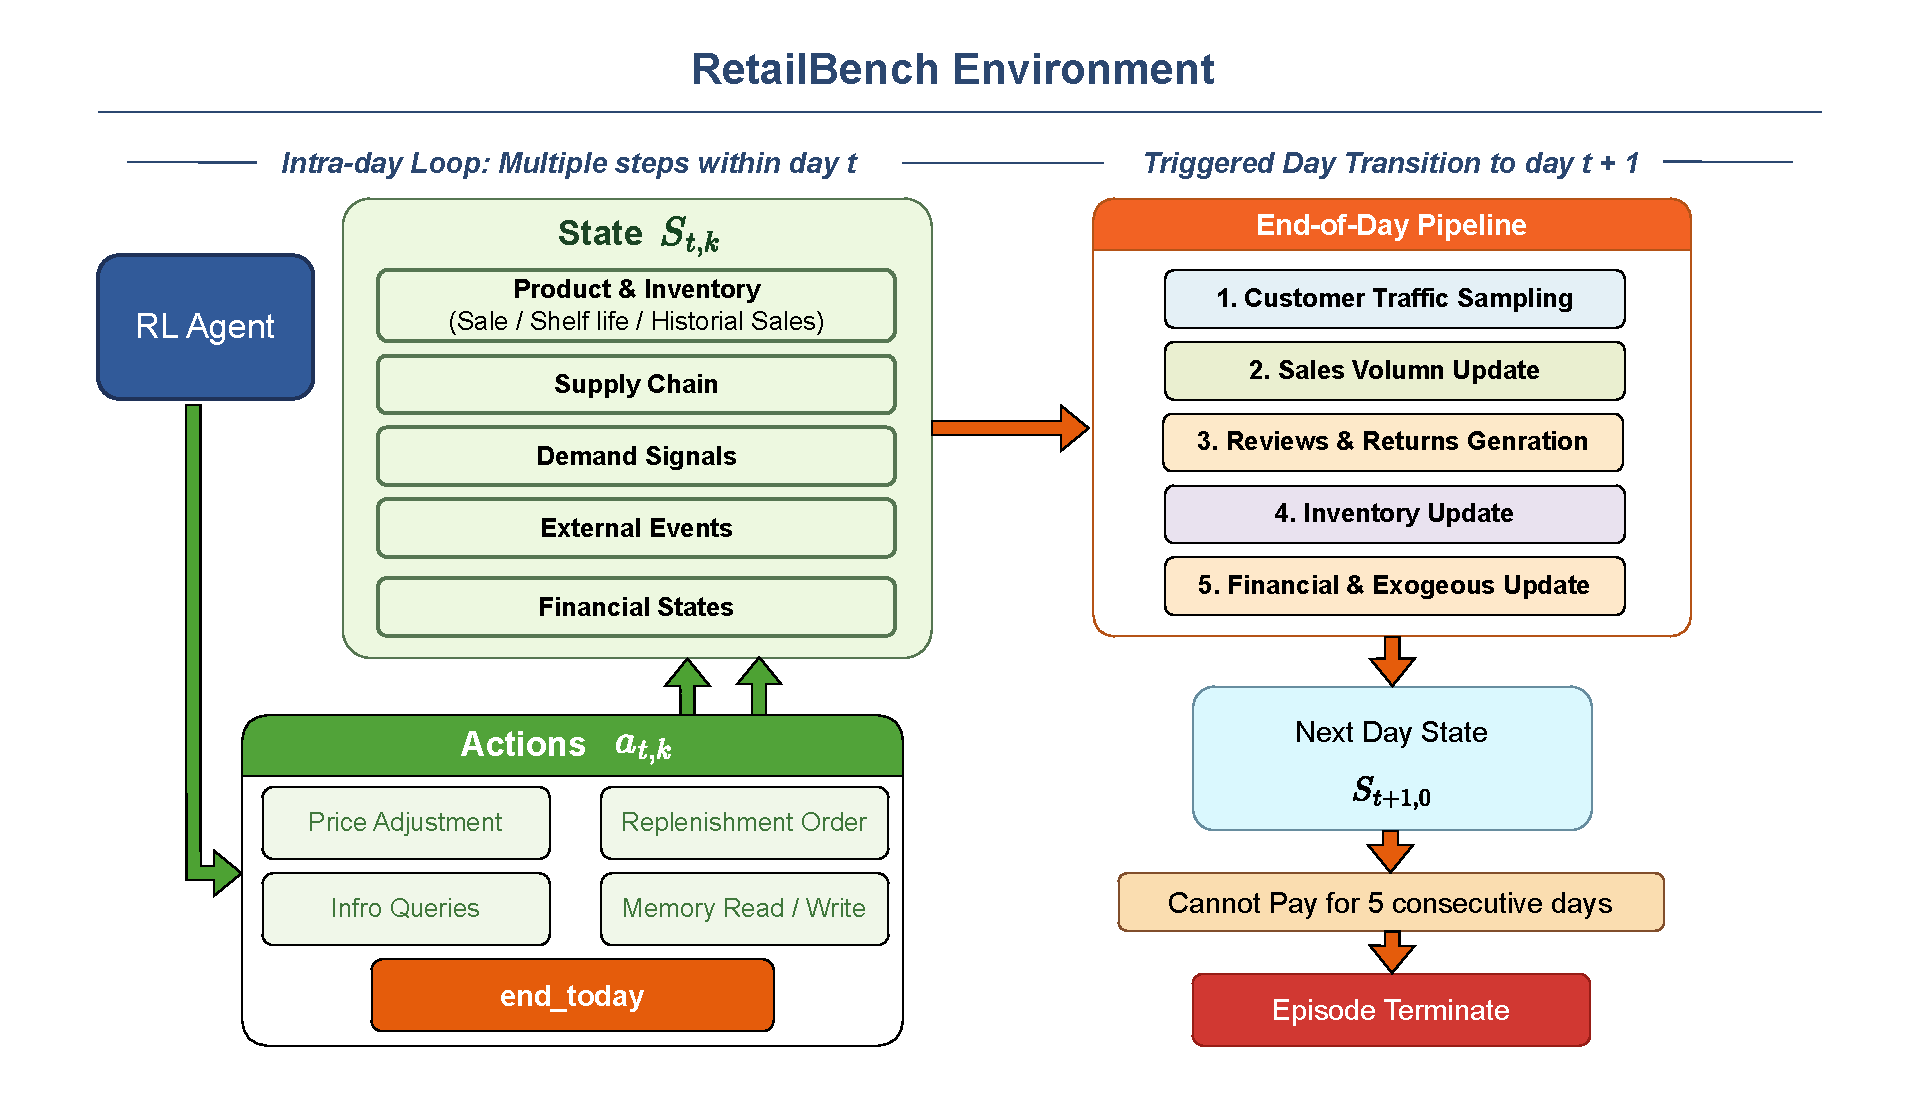
\includegraphics[width=\linewidth]{figures/env.pdf}
\end{center}
\caption{
Overview of the hierarchical supermarket environment, illustrating intra-day agent–environment interactions and end-of-day state transition dynamics.
}
\label{fig:workflow}
\vspace{-5mm}
\end{figure*}

To systematically study this challenge, we introduce \textit{RetailBench}, a benchmark that incorporates elements from retail operations and economic modeling principles. RetailBench centers on a supermarket operation scenario that demands long-horizon decision-making, sustained interaction with a dynamic environment, and the integration of heterogeneous historical information. The benchmark evaluates whether LLM-based agents can sustain business operations under stochastic, multi-factor conditions.


We evaluate eight state-of-the-art LLMs and find that current models struggle to maintain stable decisions as the decision space expands, often fail to incorporate relevant information, and frequently exhibit hallucinations and economically irrational behaviors that lead to environment collapse.

Our contributions are summarized as follows:
\begin{itemize}[leftmargin=*]
    \item We introduce \textit{RetailBench}, an open-source benchmark for evaluating long-horizon decision-making in simulated retail environments, characterized by coupled pricing-inventory control, stochastic demand, and multi-day planning horizons.
    \item Through experiments across eight models and three environment configurations, we identify and quantify four systematic failure patterns that prevent current LLM-based agents from sustaining long-horizon operations: (1) non-scalable decision-making, (2) incomplete information coverage, (3) temporal instability, and (4) invalid actions.
    \item We propose the \textit{Evolving Strategy \& Execution} framework as a reference implementation that separates high-level strategy formulation from low-level execution. In our experiments, this framework achieves improved operational stability compared to day-level Reflection baselines, though substantial gaps remain relative to heuristic policies.
\end{itemize}


\section{Environment Construction}
\label{sec:env}
\input{capter/environment_construction.tex}

\section{Evolving Strategy \& Execution Framework}
\label{sec:framework}
\subsection{Framework Detail}
\label{sec:two_stage_framework}

Prior frameworks either lack persistent strategies or revise them during execution, inducing oscillation in long-horizon settings \citep{2025planandact, yao2023react}. We propose \textit{Evolving Strategy \& Execution}, which separates strategic deliberation from operational execution. The framework maintains a persistent global strategy and restricts updates to day-level granularity to prevent excessive short-term fluctuations. In the \textit{Evolving Strategy} stage, agents examine feedback but cannot modify the environment; in the \textit{Execution} stage, strategies are fixed and immutable. This decomposition reduces strategy drift and promotes stability (illustration in Appendix~\ref{appendix:figure_framework}).

\subsection{Hierarchical Policy Representation}
\label{sec:policy}

To support structured, interpretable, and temporally extended decision-making under the proposed framework, we represent the agent policy using a hierarchical abstraction that separates strategic intent from executable actions. Each policy consists of three conceptual layers:
\begin{enumerate}[leftmargin=*]
    \item \textbf{Macro Strategy}, which captures high-level managerial objectives that persist across multiple decision steps;
    \item \textbf{Execution Strategy}, which encodes structured operational guidance in a machine-readable intermediate representation;
    \item \textbf{Daily Actions}, which specify concrete executable operations issued to the environment.
\end{enumerate}
Detailed policy configurations and example policies are provided in Appendix~\ref{appendix:policy}.


\section{Experiment Settings}
\label{sec:experiment}
\input{capter/experiment.tex}

\section{Results}
\label{sec:results}
\subsection{Performance Comparison between Agent Frameworks}

\paragraph{Interpretation guardrails.}
The following results report mean performance metrics across experimental settings with a limited number of random seeds (typically three runs per configuration). Due to stochastic demand dynamics, mixed model variants with different API versions and token budgets, and the absence of formal significance testing, reported performance differences should be interpreted as preliminary descriptive observations rather than statistically conclusive claims. Rank orderings may be sensitive to random seed selection, and effect sizes may vary with additional repetitions. Where we describe associations between framework design and performance outcomes, these reflect correlations observed in our experiments; establishing causal relationships requires controlled ablations which we leave for future work.

Due to computational budget constraints, we conduct a comprehensive four-framework comparison on three representative models: GLM-4.6, Kimi-K2 (Thinking), and GPT-5.2. As reported in Table~\ref{tab:framework_stats}, \textit{Evolving Strategy \& Execution} achieves higher mean sales and profit, and lower mean product expiration rates, compared to alternative agent frameworks in our evaluated settings\footnote{Due to computational constraints, our current evaluation uses a limited number of random seeds; we report mean performance and plan to extend with statistical significance testing in future work.}.

Based on these results, we select the two strongest-performing frameworks for broader evaluation across all eight models. When averaged over all models, our proposed framework demonstrates superior mean performance metrics relative to \textit{Reflection (Day-Level)}.

Despite these gains, a substantial gap remains relative to the hand-crafted heuristic policy, which serves as an approximate upper bound. This gap highlights the current limitations of LLM-based agents in long-horizon decision-making. Notably, Table~\ref{tab:framework_stats} also suggests that larger closed-source models, such as GPT-5.2, tend to achieve more stable and sustained store operation compared to smaller or open-source counterparts, indicating that model capacity remains an important factor alongside framework design.

Table~\ref{tab:scenario_stats} presents the complete results across all eight evaluated models. Across models, we observe recurring and systematic failure modes in the current environment, suggesting that the performance bottlenecks are structural rather than model-specific.

\begin{figure}
    \centering
    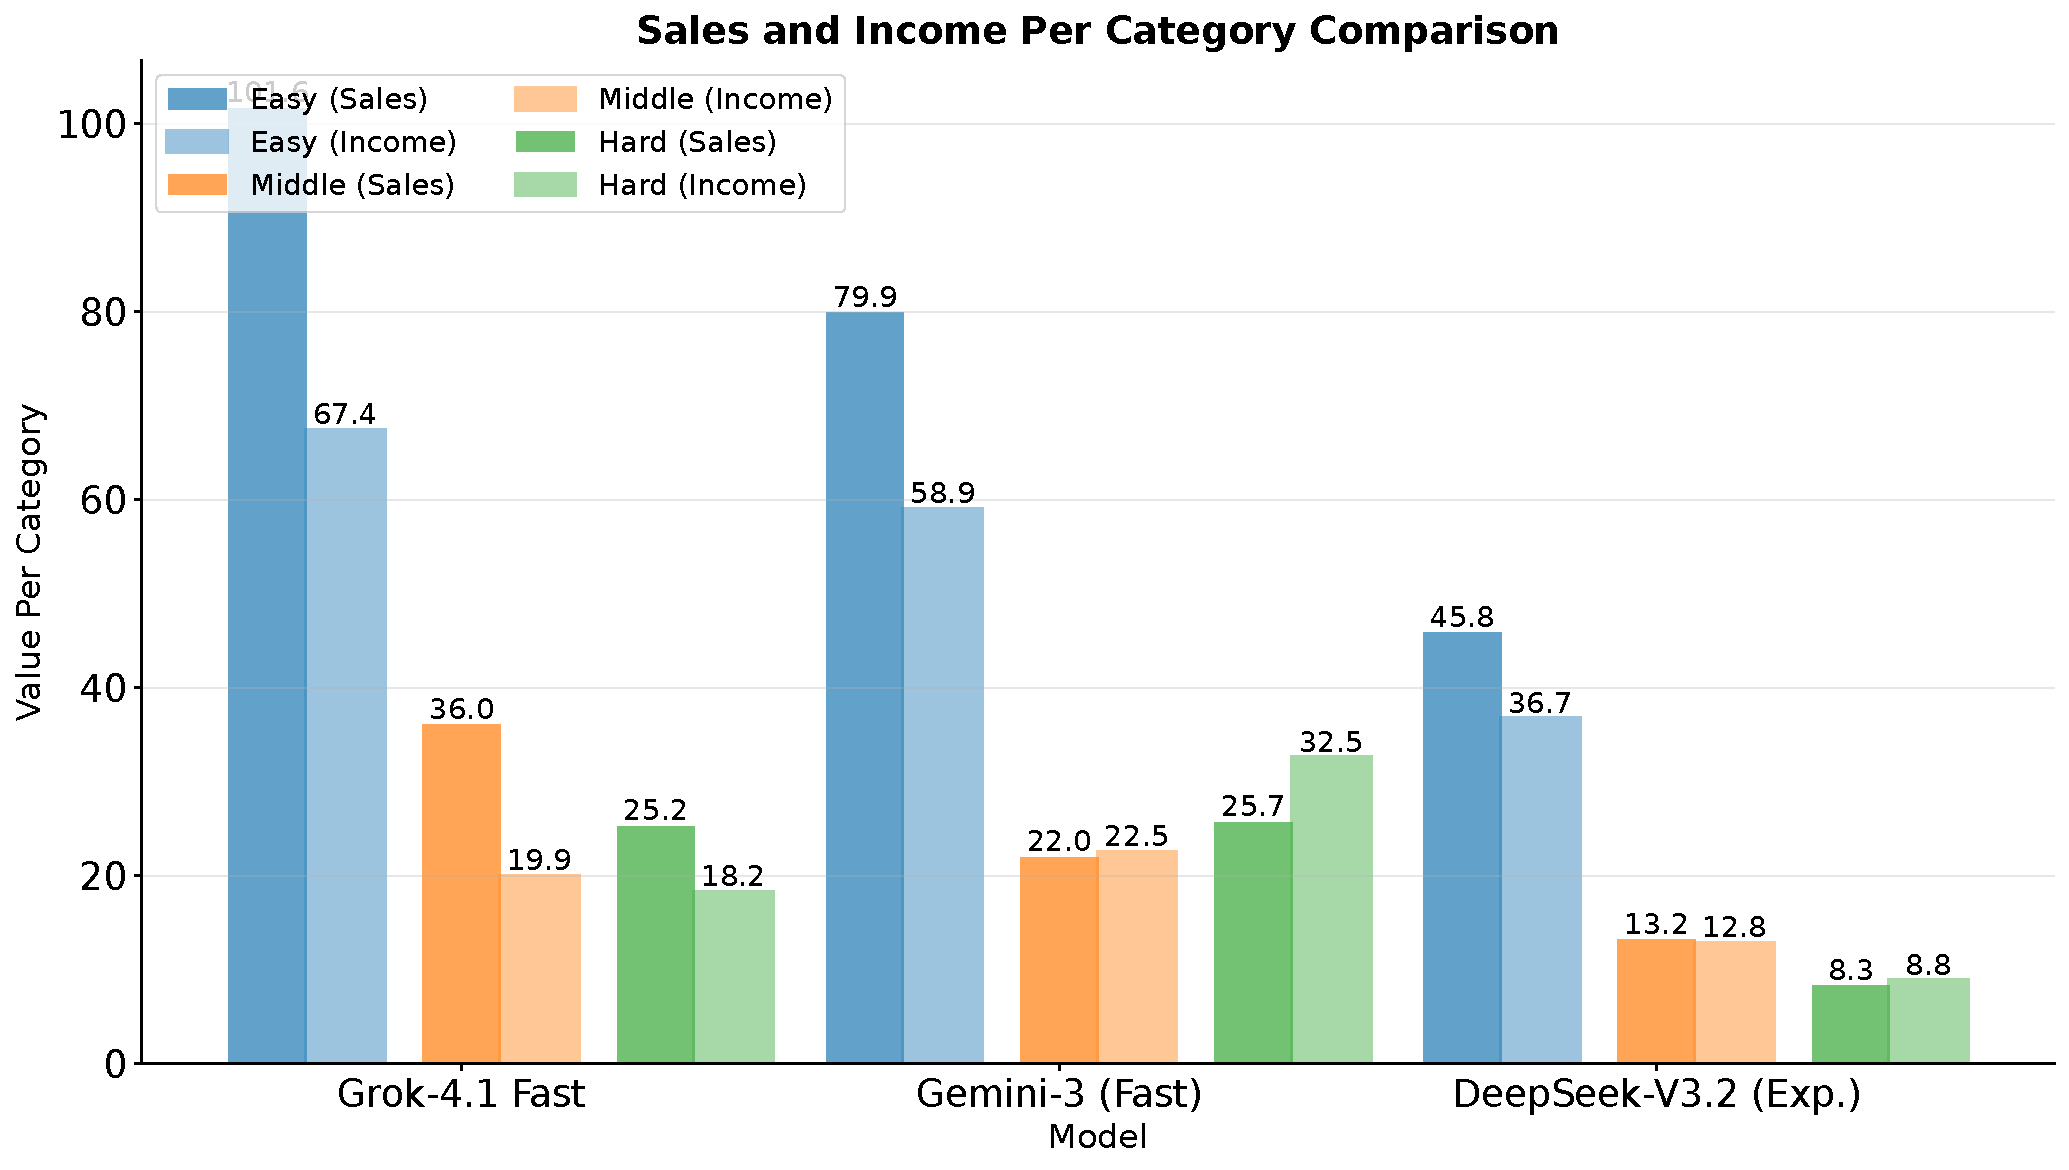
\includegraphics[width=1\linewidth]{figures/selected_models_metrics.pdf}
    \caption{Category-level sales and profit per category across Easy, Middle, and Hard environments. Results are shown for three representative models.}
    \label{fig:category_comparison}
\end{figure}

\subsection{Performance across Environments with Varying Difficulty}
As environment difficulty increases, all models exhibit consistent performance degradation in our experiments, including shorter operational durations, higher expiry and return ratios, and reduced long-horizon stability. Although the expansion of product categories in the Middle and Hard settings enables higher aggregate sales and profit for some models, \emph{Sales per Category} and \emph{Profit per Category} decline substantially (Figure~\ref{fig:category_comparison}). This pattern suggests challenges in resource allocation as decision spaces expand, though further investigation with additional seeds is needed to assess statistical significance.

The relatively small performance gap between the Middle and Hard environments can be partly attributed to the delayed impact of intensified news dynamics, whose effects typically unfold over longer time horizons. Appendix~\ref{appendix:total_results} reports the full results across all environments under the proposed framework. Overall, while models demonstrate limited adaptability as task complexity increases, their performance remains substantially below the heuristic upper bound, highlighting persistent limitations in robust long-horizon decision-making under complex and dynamic conditions.

\section{Analysis}
\label{sec:analysis}

Based on both quantitative evaluation results and manual inspection of trajectories, we identify several patterns that are associated with model failures to operate reliably in the environment in our experiments.\footnote{The analysis section presents observational patterns and correlations; causal claims about why models fail require controlled ablations which we leave for future work.}

We analyze these failure modes from four complementary perspectives.

\subsection{Non-scalable Decision-Making Capability}

\begin{table}[t]
\resizebox{\columnwidth}{!}{
\begin{tabular}{lccccccc}
\toprule
\multirow{2}{*}{\textbf{Model}} &
\multirow{2}{*}{\textbf{Context}} &
\multicolumn{2}{c}{\textbf{Easy}} &
\multicolumn{2}{c}{\textbf{Middle}} &
\multicolumn{2}{c}{\textbf{Hard}} \\
& & SKU $\uparrow$ & Cat $\uparrow$ & SKU $\uparrow$ & Cat $\uparrow$ & SKU $\uparrow$ & Cat $\uparrow$ \\
\midrule
DeepSeek-V3.2 (Exp.)
& 128K
& 4.75 & 3.31
& \underline{6.83} & \underline{5.34}
& 6.64 & \underline{5.45} \\

Gemini-3 (Fast)
& \textbf{1M}
& \textbf{8.72} & \textbf{4.34}
& \textbf{13.60} & \textbf{12.43}
& \textbf{21.57} & \textbf{13.56} \\

GLM-4.6
& 200K
& 4.82 & 2.98
& 3.23 & 2.46
& \underline{7.08} & 5.22 \\

OpenAI-5.1 Mini
& 400K
& 3.66 & 1.94
& 4.10 & 4.10
& 6.67 & 4.79 \\

Grok-4.1 Fast
& 200K
& \underline{5.78} & \underline{3.68}
& 4.87 & 3.08
& 5.40 & 3.20 \\

Kimi-K2 (Thinking)
& 256K
& 5.06 & 3.09
& 5.17 & 4.77
& 6.91 & 4.75 \\

Qwen-235B (Thinking)
& 256K
& 4.59 & 3.67
& 3.17 & 2.36
& 5.11 & 4.51 \\

\midrule
\midrule
Heuristic Strategy
& --
& 9.03 & 4.87
& 35.34 & 18.61
& 34.82 & 18.52 \\
\bottomrule
\end{tabular}
}
\caption{SKU and Category counts sold by different models across difficulties.
Context denotes the maximum supported context length of each model.
\textbf{Bolded} indicates the best model; \underline{underlined} indicates the second best (Human excluded).}
\label{tab:sold_sku_cat_context}
\vspace{-3mm}
\end{table}


As shown in Appendix~\ref{appendix:total_results}, models achieve reasonable performance in the Easy setting but exhibit consistent degradation as the environment scales in complexity. To better understand this phenomenon, we analyze both the average number of stock keeping units (SKUs) and product categories sold per day, as well as the number of SKUs and categories explicitly considered during the \emph{Evolving Strategy} phase (Tables~\ref{tab:sold_sku_cat_context} and Appendix ~\ref{appendix:category_analysis}).

Across most models, decision-making capability does not scale proportionally with the size of the environment. Instead, performance remains relatively flat despite a substantial increase in the number of available options. Notably, Gemini-3 (Fast), which supports the largest maximum context window, performs better than other models in this respect in our experiments. This pattern is consistent with the hypothesis that larger context capacity helps retain salient information even when the effective interaction context is constrained, though further investigation is needed to establish causality.

Nevertheless, even the strongest models fail to cover the full decision space in our experiments. This observation suggests that current systems may face challenges in expanding their effective decision-making scope as the environment grows, which is associated with systematic performance degradation in larger and more complex settings.

\subsection{Incomplete Decision-Making Due to Limited Information Coverage}

\begin{table}[t]
\resizebox{\columnwidth}{!}{
\begin{tabular}{lcccccccc}
\toprule
\textbf{Model} &
Supplier &
Inventory &
Return &
Rating &
Price &
Review &
Sales &
History \\
\midrule
DeepSeek-V3.2 (Exp.) & 41.4 & 100.0 & 26.7 & 75.4 & 6.6 & 0.6 & 89.2 & 0.0 \\
Gemini-3 (Fast)     & 69.6 & 100.0 & 41.0 & 82.3 & 67.7 & 6.3 & 87.6 & 2.9 \\
GLM-4.6             & 93.9 & 98.3  & 79.8 & 77.8 & 84.1 & 5.1 & 96.3 & 0.0 \\
OpenAI-5.1 Mini     & 58.8 & 99.0  & 5.1  & 78.6 & 3.9  & 10.6 & 84.7 & 0.3 \\
Grok-4.1 Fast       & 89.9 & 99.8  & 84.0 & 94.0 & 88.6 & 36.0 & 96.4 & 0.3 \\
Kimi-K2 (Thinking)  & 57.2 & 90.4  & 25.9 & 51.4 & 36.2 & 11.0 & 64.0 & 0.5 \\
Qwen-235B (Thinking)           & 76.8 & 78.3  & 31.5 & 58.2 & 19.8 & 23.6 & 74.6 & 0.0 \\
\midrule
Average             & 69.7 & 95.1  & 42.0 & 74.0 & 43.8 & 13.3 & 84.7 & 1.0 \\
\bottomrule
\end{tabular}
}
\caption{
Percentage of days on which each model queries specific information sources when making decisions for SKUs included in the final daily strategy.
Higher values indicate greater reliance on the corresponding data source.
}

\label{tab:tool_usage_easy}
\vspace{-3mm}
\end{table}


We analyze the information sources that models attend to when making operational decisions by examining the data queried for the set of SKUs included in each day’s final strategy. This analysis reveals a clear concentration of attention on a limited subset of signals.

Specifically, most models primarily rely on supplier prices, inventory levels, SKU ratings, and historical sales records when deciding how to operate selected SKUs in Table~\ref{tab:tool_usage_easy}. In contrast, several other critical signals—such as recent customer reviews, return rates, and current selling prices—are consistently underutilized or entirely ignored.



Further correlation analysis shows a positive relationship between the frequency of SKU reviews queries and average daily sales performance in Appendix~\ref{appendix:tool_use_analysis}. This observation aligns with the underlying environment dynamics and is consistent with incomplete information coverage being a factor associated with lower decision quality in our experiments. Overall, these results suggest that models often fail to perform sufficiently comprehensive information gathering, which is correlated with suboptimal operational decisions.
% \begin{table}[t]
% \resizebox{\columnwidth}{!}{
% \begin{tabular}{lccccccc}
% \toprule
% \multirow{2}{*}{\textbf{Model}} &
% \multirow{2}{*}{\textbf{Context}} &
% \multicolumn{2}{c}{\textbf{Easy}} &
% \multicolumn{2}{c}{\textbf{Middle}} &
% \multicolumn{2}{c}{\textbf{Hard}} \\
% & & SKU & Cat & SKU & Cat & SKU & Cat \\
% \midrule
% DeepSeek-V3.2 (Exp.)
% & 128K
% & 7.80 & \underline{4.07}
% & 6.43 & 4.25
% & 4.71 & 3.65 \\

% Gemini-3 (Fast)
% & \textbf{1M}
% & \textbf{8.50} & 3.95
% & \textbf{11.89} & \textbf{11.18}
% & \textbf{13.32} & \textbf{8.09} \\

% GLM-4.6
% & 200K
% & 6.61 & 3.55
% & 6.01 & 3.48
% & \underline{8.47} & \underline{6.05} \\

% OpenAI-5.1 Mini
% & 400K
% & 6.80 & 2.64
% & \underline{6.82} & \underline{6.81}
% & 7.87 & 5.19 \\

% Grok-4.1 Fast
% & 200K
% & \underline{7.88} & \textbf{4.35}
% & 6.51 & 3.53
% & 7.69 & 3.90 \\

% Kimi-K2 (Thinking)
% & 256K
% & 5.92 & 2.94
% & 5.53 & 4.09
% & 6.03 & 3.22 \\

% Qwen-235B
% & 256K
% & 4.78 & 3.66
% & 6.49 & 4.05
% & 5.77 & 4.23 \\

% \midrule
% \midrule
% Heuristic Strategy
% & --
% & - & -
% & - & -
% & - & - \\
% \bottomrule
% \end{tabular}
% }
% \caption{SKU and Category counts observed during the strategy stage across difficulties.
% Context denotes the maximum supported context length of each model.
% \textbf{Bolded} indicates the best model; \underline{underlined} indicates the second best (Heuristic Strategy excluded).}
% \label{tab:strategy_sku_cat_context}
% \vspace{-3mm}
% \end{table}



\begin{table}[t]
\centering
\small
\resizebox{\columnwidth}{!}{%
\begin{tabular}{lcccccc}
\toprule
 & \multicolumn{3}{c}{\textbf{Macro Strategy}} 
 & \multicolumn{3}{c}{\textbf{Execution Strategy}} \\
\cmidrule(lr){2-4} \cmidrule(lr){5-7}
\textbf{Model} 
& Std\_diff~(↓) & MAC~(↓) & TV~(↓)
& Std\_diff~(↓) & MAC~(↓) & TV~(↓) \\
\midrule
DeepSeek-V3.2(Exp.)  
& 0.130 & 0.090 & 5.00 
& 0.289 & 0.144 & 7.93 \\
Gemini-3 (Fast)    
& 0.136 & 0.085 & 3.82 
& 0.293 & 0.225 & 10.18 \\
GLM-4.6          
& 0.131 & 0.096 & 4.52 
& 0.264 & 0.209 & 9.87 \\
OpenAI-5.1 Mini       
& 0.069 & 0.051 & 2.50 
& 0.229 & 0.166 & 8.00 \\
Grok-4.1 Fast    
& 0.079 & 0.045 & 2.71 
& 0.204 & 0.151 & 9.39 \\
Kimi K2(Thinking)
& 0.179 & 0.133 & \textbf{6.95} 
& 0.335 & 0.271 & \textbf{14.08} \\
Qwen-235B (Thinking)        
& \textbf{0.240} & \textbf{0.189} & 6.51 
& \textbf{0.391} & \textbf{0.306} & 10.57 \\
\bottomrule
\end{tabular}
}

\caption{Temporal instability metrics of macro- and execution-level strategy similarity in the Easy environment. All metrics are lower-is-better (↓). Larger values indicate greater temporal instability. Column-wise maximum values are highlighted in bold.}
\label{tab:strategy_instability_easy}
\end{table}
\subsection{Temporal Instability in Execution-Level Decision-Making}

Beyond limitations in decision scalability and information coverage, we observe temporal instability in execution-level decision-making which is associated with long-horizon failures in our experiments. Even under relatively stable environmental conditions, agents frequently revise their strategies across consecutive days, resulting in inconsistent execution trajectories.

\paragraph{Measuring Strategy Similarity.}
We quantify temporal instability by measuring the similarity between strategies on adjacent days at both macro and execution levels. Macro strategy similarity is assessed using an LLM-based prompt that evaluates semantic consistency between consecutive high-level plans. Execution strategy similarity is computed via set-based Jaccard similarity over key fields, including \texttt{focus\_skus}, \texttt{sku\_supplier\_mapping}, \texttt{news\_to\_monitor}, and \texttt{sku\_to\_monitor}, with the final execution similarity obtained by averaging across fields.

\paragraph{Instability Metrics.}
To characterize temporal fluctuations, we compute three complementary metrics: the standard deviation of first-order differences (\textit{Std\_diff}) to capture short-term volatility, the mean absolute change (\textit{MAC}) to estimate typical day-to-day variation, and total variation (\textit{TV}) to reflect cumulative long-term instability.

Across all three environment configurations, we observe consistent temporal instability in both macro- and execution-level strategies. For clarity, we present detailed results from the Easy environment in Table~\ref{tab:strategy_instability_easy} and Appendix~\ref{appendix:score_analysis} . Despite its reduced complexity, the Easy setting already exhibits pronounced temporal fluctuations. In particular, macro strategies remain relatively stable over time, whereas execution strategies show substantially larger variability across most models. This effect is especially pronounced for Qwen-235B (Thinking), which also performs poorly across all environments.

Overall, these results suggest that long-horizon failures in our experiments are associated not only with suboptimal strategy formulation, but also with the inability to maintain temporally consistent execution policies over extended horizons. Causal attribution requires controlled ablations which we leave for future work.
\subsection{Hallucinations and Invalid Actions}

Finally, manual inspection reveals recurrent failure patterns that directly break planning correctness and action validity. We distinguish two closely related but practically different issues:

\paragraph{Hallucinations in reasoning}
Models occasionally generate reasoning traces that reference non-existent SKUs or fabricate numerical quantities, and subsequently incorporate these hallucinated elements into multi-step plans (examples are provided in Appendix~\ref{appendix:hallucinations}). As a result, decisions become misaligned with the true environment state, even when the overall planning structure appears internally coherent.

  
\paragraph{Invalid or irrational actions.}
Models sometimes output actions that violate basic constraints or are inconsistent with historical demand, such as negative order quantities or implausible pricing in Appendix~\ref{appendix:invalid_action}. Even though state-modifying operations are restricted to only a small set of tools, these invalid actions occur with non-negligible frequency and can quickly destabilize the system in long-horizon operation.

In realistic operational settings, both hallucinations and invalid actions would be unacceptable and could directly trigger system collapse.



\section{Related Work}
\label{sec:related_work}
% \paragraph{Retail and supply-chain decision benchmarks.}
% Recent work on retail and supply-chain decision-making has evolved from isolated subproblems toward integrated, multi-stage environments. Reinforcement-learning benchmarks such as OFCOURSE, GymSC-style simulators, and MARLIM \citep{OFCOURSE, inventory, leluc2023marlimmultiagentreinforcementlearning} model fulfillment and inventory control under demand uncertainty, demonstrating the effectiveness of learned policies in mitigating effects such as demand volatility. However, these environments typically emphasize fixed structures and short- to medium-horizon policies, limiting their ability to evaluate sustained strategic behavior. More recent benchmarks incorporating LLM-based agents, including InvAgent and AIM-Bench \citep{invagentlargelanguagemodel, aimbenchevaluatingdecisionmakingbiases}, begin to explore language-driven reasoning and decision biases, yet still fall short in assessing long-horizon, strategy-aware autonomy in realistic retail settings.

\paragraph{Long-horizon planning benchmarks for LLMs.}
In parallel, a growing body of benchmarks targets long-horizon planning abilities of large language models across structured and interactive environments. PlanBench focuses on classical plan generation, while WebShop, Mind2Web, and ScienceWorld \citep{mind2web, scienceworldagentsmarter5th, 3webshopscalablerealworldweb} evaluate multi-step interaction, error recovery, and adaptive behavior in dynamic settings. More recent benchmarks---such as HeroBench, OdysseyBench, UltraHorizon \citep{utltabench, herobenchbenchmarklonghorizonplanning, odysseybenchevaluatingllmagents}, and explicitly stress extended, interdependent decision sequences that require persistent memory, hierarchical reasoning, and long-term strategy maintenance. Collectively, these benchmarks suggest that while short-horizon tasks are increasingly tractable, robust long-horizon planning and execution remain a central challenge for LLM-based agents.

\paragraph{Long-horizon agent frameworks.}
Recent advances in agent design address these challenges by introducing structured frameworks that decouple high-level planning from low-level execution. Approaches such as Plan-and-Act \citep{erdogan2025planandactimprovingplanningagents} and EAGLET \citep{si2025goalplanjustwish} adopt planner--executor architectures to support hierarchical decision-making, dynamic replanning, and improved execution stability over long horizons. Extensions to multi-agent settings ELHPlan \citep{ling2025elhplanefficientlonghorizontask} and plan-aware context management frameworks PAACE \citep{yuksel2025paaceplanawareautomatedagent} further emphasize task decomposition, explicit strategy representation, and memory-aware context control. Together, these works indicate that scalable long-horizon autonomy increasingly relies on structured planning modules and controlled execution mechanisms rather than monolithic end-to-end policies.

\paragraph{Positioning relative to existing benchmarks.}
RetailBench complements existing benchmarks by targeting a specific combination of properties not jointly addressed in prior work: (1) long-horizon planning over multi-day episodes with day-level decisions, (2) economic optimization objectives (profit maximization under inventory and pricing constraints), (3) coupled decision spaces where pricing affects inventory turnover and vice versa, (4) stochastic dynamics from demand uncertainty, news shocks, and supply-chain delays, and (5) open-source availability for reproducible evaluation. While benchmarks such as WebArena and Mind2Web evaluate multi-step tool use, and VendingBench and OdysseyBench assess long-horizon planning, RetailBench is distinguished by its focus on economically grounded retail operations with realistic temporal dependencies and delayed rewards. Table~\ref{tab:novelty_comparison} provides a detailed comparison.

\begin{table}[t]
\centering
\small
\caption{Comparison of RetailBench with related long-horizon benchmarks. Horizon length is measured in typical decision steps. Economic objective refers to explicit profit/cost optimization. Open-source indicates public simulator availability. \footnotesize{\textit{Note: Horizon categories are approximate based on cited papers; cross-domain horizons are not directly comparable due to different task structures and step definitions.}}}
\label{tab:novelty_comparison}
\begin{tabular}{lcccc}
\toprule
Benchmark & Domain & Horizon & Economic Obj. & Open Source \\
\midrule
WebArena~\citep{webarenarea} & Web tasks & Short ($<50$) & No & Yes \\
Mind2Web~\citep{mind2web} & Web tasks & Medium ($50$-$200$) & No & Yes \\
VendingBench~\citep{andonlabs2025vendingbench2} & Vending & Long ($200+$) & Limited & Yes \\
OdysseyBench~\citep{odysseybenchevaluatesllmagents} & Games & Long ($200+$) & No & Yes \\
\textbf{RetailBench} & \textbf{Retail Ops.} & \textbf{Long ($200+$)} & \textbf{Yes} & \textbf{Yes} \\
\bottomrule
\end{tabular}
\end{table}

\section{Conclusion}
\label{sec:conclusion}
This paper introduces RetailBench, a benchmark for evaluating long-horizon decision-making in simulated retail environments. RetailBench models supermarket operations as a stochastic, multi-factor, and temporally extended process, requiring agents to reason jointly about pricing, inventory, information acquisition, and financial sustainability. We further propose the Evolving Strategy \& Execution framework, which decouples high-level strategy evolution from low-level execution to better support long-horizon autonomy.

Experiments on eight state-of-the-art large language models show that, in our evaluated settings, our framework achieves higher mean operational stability and economic performance metrics compared to day-level Reflection baselines. However, performance degrades sharply as environment complexity increases, and all models remain substantially below heuristic upper bounds. These results suggest that while structured agent frameworks mitigate some challenges, current LLM-based agents face persistent difficulties in scalability, information use, execution stability, and action validity within the RetailBench environment. Whether these limitations generalize to other domains remains an open question for future research. RetailBench thus provides a principled testbed for advancing research on long-horizon decision-making and agentic reasoning.

\section{Limitations}
\label{sec:limitation}
\section*{Limitations}

Our work has several important limitations. First, our evaluation is conducted in a simulated single-store environment; external validity beyond this setting remains to be established. Second, due to computational constraints, we use only three runs per model without formal significance testing—reported differences are preliminary observations rather than statistically significant conclusions. Third, our baselines exclude classical operations research methods (e.g., newsvendor policies, dynamic pricing); the relative performance of LLM-based agents against these well-established methods remains unknown. Finally, we evaluate zero-shot prompting without learning; stronger performance may be achievable through fine-tuning or reinforcement learning.


% \subsection{Results of different agent framework}
% 我们在easy 环境下对于所有模型进行的三次实验,并通过


% \subsection{Results of different environment framework}





% \subsection{为什么模型无法成功运行店铺}
% 我们从实验的结果中
% \subsection{模型是否能够根据环境反馈做出策略调整}
% \subsection{模型的策略调整有多少是有效的,合理的}


% Bibliography entries for the entire Anthology, followed by custom entries
%\bibliography{anthology,custom}
% Custom bibliography entries only
\bibliography{custom}

\appendix
\section{Environment Configuration Details}
\label{appendix:env_details}
\input{capter/appendix_a.tex}


\section{Rollout Details}
\label{appendix:rollout_obs}
\input{capter/appendix_b.tex}

\section{Prompt}
\label{appendix:prompt}
\subsection{Evolving Strategy \& Execution Framework Evolving Strategy Phase System Prompts}

\begin{Verbatim}[breaklines=true, breakanywhere=true]
You are a retail strategy analyst. Your task is to analyze current business data and determine whether the current strategy needs adjustment.


Environment Characteristics

- The store operates with a large number of SKUs, where products within the same category interact and may substitute or cannibalize each other's demand.
- Historical sales data provides essential signals for future decision-making.
- Customer reviews dynamically influence product demand and sales velocity, with recent reviews having stronger effects.
{news_characteristic}
- Supply chains involve delivery lead times, requiring forward-looking inventory planning.
- Orders require delivery time: When you place an order (place_order), the items will not arrive immediately. The delivery time varies and can take up to 7 days (within 7 days). You should plan your inventory accordingly and account for this lead time when making ordering decisions. Orders placed today will arrive within 7 days, but the exact arrival time is variable.
- Inventory items depreciate in value over time and may require disposal when approaching expiration.
- Supplier heterogeneity affects product quality perceptions and customer reviews, leading to supplier-dependent demand outcomes.
- Daily rent: The store incurs a fixed daily rent cost of {daily_rent} that must be paid each day. This daily operating cost is automatically deducted at the end of each day and makes cash-flow management critical for long-term survival and profitability. You must ensure sufficient funds are available to cover the daily rent. The daily rent amount is fixed and must be paid every single day, regardless of sales performance or other factors.

# Your Role in Strategy Phase

Each day starts with a STRATEGY PHASE where you:
1. Review the current strategy (provided at the start of this phase)
2. Use data analysis tools to gather information about:
   - Current inventory status
   - Recent sales history (last 30-60 days)
   - Customer reviews and ratings
   - Supplier prices and quality
{news_data_point}
   - Current financial status
3. Compare current situation with previous days to identify significant changes
4. Set the strategy using the three separate tools (set_macro_strategy, set_execute_strategy, set_action) to set the three strategy components

# Strategy Format

The strategy consists of three components:

1. **macro_strategy**: A list of broad strategic guidelines (array of strings)
   - Examples: ["Focus on high-margin products", "Maintain competitive pricing", "Prioritize inventory turnover"]

2. **execute_strategy**: An object with seven fields, all values are arrays:
   - **focus_skus**: Array of SKU IDs that need attention (e.g., ["SKU_001", "SKU_002"])
   - **sku_supplier_mapping**: Array of mapping objects (e.g., [{{"sku_id": "SKU_001", "supplier_id": "supplier_A"}}, {{"sku_id": "SKU_002", "supplier_id": "supplier_B"}}])
{news_to_monitor_field}
   - **skus_to_reorder**: Array of SKU IDs that need reordering (e.g., ["SKU_003", "SKU_004"])
   - **price_adjustments**: Array of price adjustment objects (e.g., [{{"sku_id": "SKU_001", "adjustment": "increase by 10%"}}, {{"sku_id": "SKU_002", "adjustment": "decrease by 5%"}}])
   - **sku_to_monitor**: Array of SKU IDs that should be closely monitored (e.g., ["SKU_005", "SKU_006"])
   - **other**: Array of other strategy notes or metadata (e.g., [{{"comment": "..."}}, {{"risk_level": "high"}}])

3. **today_action**: An array of action objects, each representing a concrete action using the parameter format of `place_order` or `modify_sku_price`.
   - Each action MUST be an object of the form:
     - {{"tool": "place_order", "arguments": }}
     - OR {{"tool": "modify_sku_price", "arguments": }}
   - Example:
     [
       {{"tool": "place_order", "arguments": {{"sku_id": "SKU_001", "supplier_id": "supplier_A", "quantity": 100}}}},
       {{"tool": "modify_sku_price", "arguments": {{"sku_id": "SKU_002", "new_price": 9.99}}}}
     ]

# Strategy Setting Tools

Use three separate tools to set different parts of the strategy:
- **set_macro_strategy**: Set the macro_strategy (array of strings)
  - Parameter: `macro_strategy` (array of strings)
  - Example: set_macro_strategy(macro_strategy=["Focus on high-margin products", "Maintain competitive pricing"])

- **set_execute_strategy**: Set the execute_strategy (object with seven fields, all arrays)
  - Parameter: `execute_strategy` (object with fields: focus_skus, sku_supplier_mapping{news_to_monitor_param}, skus_to_reorder, price_adjustments, sku_to_monitor, other)
  - All field values must be arrays
  - Example: set_execute_strategy(execute_strategy={{"focus_skus": ["SKU_001"], "sku_supplier_mapping": [{{"sku_id": "SKU_001", "supplier_id": "supplier_A"}}], ...}})

- **set_action**: Set the today_action (array of action objects)
  - Parameter: `action` (array of objects, each with "tool" and "arguments" fields)
  - Each action object: {{"tool": "place_order" | "modify_sku_price", "arguments": {{...}}}}
  - Example: set_action(action=[{{"tool": "place_order", "arguments": {{"sku_id": "SKU_001", "supplier_id": "supplier_A", "quantity": 100}}}}])

You can call these tools multiple times to build or modify the strategy. After your analysis, set all three components to reflect your decisions.

# Available Tools for Analysis

The available function signatures are provided within <tools></tools> XML tags:
<tools>
{tool_definitions}
</tools>

For each function call, return a JSON object with function name and arguments inside <tool_call></tool_call> XML tags:
<tool_call>
{{"name": <function-name>, "arguments": <args-json-object>}}
</tool_call>

# Important Analysis Tools

Use these tools to gather data:
- view_funds_and_date: Check current funds and date
- view_inventory: Check current inventory levels
- view_sku_sales_history: Analyze sales trends (use last 30-60 days)
- view_sku_avg_ratings: Check customer satisfaction
- view_current_date_supplier_prices: Check supplier availability and prices
{news_tools_list}
- view_current_orders: Check pending orders
- set_macro_strategy: Set the macro strategy (array of strings)
- set_execute_strategy: Set the execute strategy (object with seven fields, all arrays)
- set_action: Set the today action (array of action objects)

Note: You CANNOT use place_order or modify_sku_price in the strategy phase. These tools are only available in the execution phase.

After completing your analysis and updating the strategy, the system will transition to the EXECUTION PHASE.
\end{Verbatim}

\subsection{Evolving Strategy \& Execution Execution Framework Phase System Prompts}

\begin{Verbatim}[breaklines=true, breakanywhere=true]
You are a retail operations agent executing daily operations based on the current strategy.

# Your Role in Execution Phase

In the EXECUTION PHASE, you will receive the **final strategy** determined in the Strategy Phase. This strategy includes:
- **macro_strategy**: Broad strategic guidelines (array of strings)
- **execute_strategy**: Specific operational details (object with seven fields, all arrays)
- **today_action**: Concrete actions to take today (array of action objects)

# Important Operational Constraints

- **Daily rent**: The store incurs a fixed daily rent cost of {daily_rent} that must be paid each day. This daily operating cost is automatically deducted at the end of each day. Ensure you have sufficient funds to cover this daily expense. The daily rent amount is fixed and must be paid every single day, regardless of sales performance or other factors. This makes cash-flow management critical for long-term survival and profitability.
- **Order delivery time**: When you place an order using place_order, the items will not arrive immediately. The delivery time varies and can take up to 7 days (within 7 days). Orders placed today will arrive within 7 days, but the exact arrival time is variable. Plan your inventory and ordering decisions accordingly, considering the lead time for items to arrive.

# Strategy Usage Guidelines

**The strategy is provided as REFERENCE, but you can and should make additional actions based on real-time data:**

1. **Reference the strategy** to understand priorities and planned actions:
   - Use macro_strategy for overall decision-making direction
   - Use execute_strategy fields (focus_skus, sku_supplier_mapping{news_to_monitor_ref}, skus_to_reorder, price_adjustments, sku_to_monitor, other) as guidance
   - Consider today_action as suggested actions to take

2. **Perform additional data queries** to validate and refine decisions:
   - Check current inventory levels, sales history, supplier prices{news_impacts_ref}, funds, etc.
   - Use tools like view_inventory, view_sku_sales_history, view_current_date_supplier_prices{news_tools_ref}, etc.

3. **Execute actions flexibly**:
   - You can execute actions from today_action when they still make sense given the latest data
   - You can **adjust, skip, or modify** actions from today_action if your analysis shows better alternatives
   - You can **add additional actions** beyond today_action if needed (e.g., unexpected inventory changes, new supplier prices{news_impacts_example})
   - You can use information from execute_strategy (like focus_skus, sku_supplier_mapping) to make decisions even if not explicitly in today_action

4. **End the day** by calling end_today when you've completed all operations for today.

# Important Constraints

- You MUST NOT modify the stored strategy itself in this phase (strategy can only be changed in the Strategy Phase)
- You CANNOT call any tool that changes macro_strategy / execute_strategy / today_action
- You SHOULD use the strategy as guidance but make final decisions based on current data and analysis

# Available Tools

The available function signatures are provided within <tools></tools> XML tags:
<tools>
{tool_definitions}
</tools>

For each function call, return a JSON object with function name and arguments inside <tool_call></tool_call> XML tags:
<tool_call>
{{"name": <function-name>, "arguments": <args-json-object>}}
</tool_call>

# Ending the Day

When you have completed all reasonable operations for the day (especially those in today_action, adjusted as needed by current data), you MUST call end_today to advance to the next day. This will trigger a new Strategy Phase for the next day.
\end{Verbatim}

\subsection{Reflection Framework Reflection Phase Prompts}

\begin{Verbatim}[breaklines=true, breakanywhere=true]
This prompt is used to generate reflections after each day in \texttt{run\_reflection.py}.

\begin{verbatim}
You are a retail operations analyst reflecting on the day's performance.

# Task Goal
{task_spec}

# Day {day} End Result
{end_today_result.get('formatted', safe_dump(end_today_result))}

# Day {day} Interaction History
{interaction_summary}
{memory_context}

# Your Task

Generate a comprehensive reflection on today's performance. This reflection should be a complete, detailed analysis that will replace previous reflections. Include:

1. **Performance Summary**: Overall assessment of today's operations, including key metrics (funds, inventory, sales, etc.)

2. **Issue Identification**: What specific problems or challenges occurred? Be specific about what went wrong.

3. **Root Cause Analysis**: Why did these problems happen? Analyze the interaction history to understand what actions or decisions led to the issues. Trace back through the day's operations.

4. **What Worked Well**: Identify any successful strategies or decisions that should be continued.

5. **Actionable Improvements**: What should be done differently next time? Provide specific, actionable recommendations for future operations.

6. **Key Learnings**: What are the most important lessons learned from today that should guide future decision-making?

Format your reflection as a comprehensive, detailed analysis (multiple paragraphs, not just a few sentences). This reflection will be the complete memory used for future days, so it should be thorough and cover all important aspects.

Reflection:
\end{Verbatim}




\subsection{Macro Similiarity Judge Prompt}

\begin{Verbatim}[breaklines=true, breakanywhere=true]
Please compare the similarity of the following two macro strategies.

Strategy 1's macro_strategy:
{macro1_formatted}

Strategy 2's macro_strategy:
{macro2_formatted}

Please evaluate the similarity between these two strategies and provide a score between 0 and 1, where:
- 1.0 means identical or almost identical
- 0.8-0.9 means very similar with only minor differences
- 0.6-0.7 means somewhat similar with some common points
- 0.4-0.5 means somewhat similar but with significant differences
- 0.2-0.3 means not very similar
- 0.0-0.1 means completely different

Please return only a floating-point number between 0 and 1, without any additional text or explanation.
\end{Verbatim}





\section{Agent Framework}
\label{appendix:agent_framework}
\input{capter/appendix_d.tex}

\end{document}